% -*- latex -*-
%%%%%%%%%%%%%%%%%%%%%%%%%%%%%%%%%%%%%%%%%%%%%%%%%%%%%%%%%%%%%%%%
%%%%%%%%%%%%%%%%%%%%%%%%%%%%%%%%%%%%%%%%%%%%%%%%%%%%%%%%%%%%%%%%
%%%%
%%%% This text file is part of the source of 
%%%% `Introduction to High-Performance Scientific Computing'
%%%% by Victor Eijkhout, copyright 2012-2022
%%%%
%%%% This book is distributed under a Creative Commons Attribution 3.0
%%%% Unported (CC BY 3.0) license and made possible by funding from
%%%% The Saylor Foundation \url{http://www.saylor.org}.
%%%%
%%%%
%%%%%%%%%%%%%%%%%%%%%%%%%%%%%%%%%%%%%%%%%%%%%%%%%%%%%%%%%%%%%%%%
%%%%%%%%%%%%%%%%%%%%%%%%%%%%%%%%%%%%%%%%%%%%%%%%%%%%%%%%%%%%%%%%

\Level 0 {File types in programming}

\begin{purpose}
  In this section you will be introduced to the different types of
  files that you encounter while programming.
\end{purpose}

\Level 1 {Introduction to file types}

Your file system has many files, and for purposes of programming
we can roughly divide them into `text file', which are readable to you,
and `binary files', which are not meaningfully readable to you,
but which make sense to the computer.

The unix command \indextermunix{file} can tell you what type
of file you are dealing with.
\begin{verbatim}
$$ file README.txt
README.txt: ASCII text
$$ mkdir mydir
$$ file mydir
mydir: directory
$$ which ls  
\end{verbatim}

This command can also tell you about binary files.
Here the output differs by operating system.
\begin{verbatim}
$$ which ls
/bin/ls

# on a Mac laptop:
$$ file /bin/ls
/bin/ls: Mach-O 64-bit x86_64 executable

# on a Linux box
$$ file /bin/ls
/bin/ls: ELF 64-bit LSB executable, x86-64
\end{verbatim}

\begin{exercise}
  Apply the \indextermunix{file} command to sources for different programming
  language. Can you find out how \indextermunix{file} figures things out?
\end{exercise}

In figure~\ref{fig:file-types} you find a brief summary of file types.
We will now discuss them in more detail.

\begin{figure}[ht]
  \begin{tabular}{|l|l|}
    \midrule
    \multicolumn{2}{|c|}{Text files}\\
    \midrule
    Source&Program text that you write\\
    Header&also written by you, but not really program text.\\
    \midrule
    \multicolumn{2}{|c|}{Binary files}\\
    \midrule
    Object file&The compiled result of a single source file\\
    Library&Multiple object files bundled together\\
    Executable&Binary file that can be invoked as a command\\
    Data files&Written and read by a program\\
    \midrule
  \end{tabular}
  \caption{Different types of files.}
  \label{fig:file-types}
\end{figure}

\Level 1 {About `text' files}

Readable files are sometimes called \indextermsub{text}{file}s;
but this is not a concept with a hard definition.
One not-perfect definition is that text files are \indexterm{ascii} files,
meaning files where every byte uses `7-bit ascii': the first bit of every
byte is~zero.

This definition is incomplete, since modern programming languages
can often use \indexterm{unicode}, at least in character strings.
(For a tutorial on ascii and unicode, see chapter~6
of~\cite{Eijkhout:TeXscience}.)

\Level 1 {Source versus program}

There are two types of programming languages:
\begin{enumerate}
\item In an \indextermsubdef{interpreted}{language} you write
  human-readable source code and you execute it directly: the computer
  translates your source line by line as it encounters it. 
\item In a \indextermsubdef{compiled}{language} your code whole source
  is first compiled to a program, which you then execute.
\end{enumerate}
Examples of interpreted languages are \indexterm{Python},
\indexterm{Matlab}, \indexterm{Basic}, \indexterm{Lisp}.
Interpreted languages have some advantages: often you can write them
in an interactive environment that allows you to test code very
quickly. They also allow you to construct code dynamically, during
runtime. However, all this flexibility comes at a price: if a source
line is executed twice, it is translated twice. In the context of this
book, then, we will focus on compiled languages, using \indexterm{C}
and \indexterm{Fortran} as prototypical examples.

So now you have
a distinction between the readable source code, and the
unreadable, but executable, program code. In this tutorial you will
learn about the translation process from the one to the other. The
program doing this translation is known as a \indextermdef{compiler}.
This tutorial will be a `user manual' for compilers, as it were; what
goes on inside a compiler is a different branch of computer science.

\Level 1 {Binary files}

Binary files fall in two categories:
\begin{itemize}
\item executable code,
\item data
\end{itemize}

Data files can be really anything: they are typically output from
a program, and their format is often specific to that program,
although there are some standards, such as \indexterm{hdf5}.
You get a binary data file if you write out the exact bytes
of certain integers or floating point numbers,
rather than a readable representation of that number.

\begin{exercise}
  Why don't programs write their results to file in readable form?
\end{exercise}

\begin{enrichment}
  How do you write/read a binary file in C and Fortran?
  Use the function \indextermunix{hexdump} to make sense
  of the binary file.
  Can you generate the file from Fortran, and read it from~C?
  (Answer: yes, but it's not quite straightforward.)
  What does this tell you about binary data?

\end{enrichment}

In this tutorial you will mostly be concerned with executable binary files.
We then distinguish between:
\begin{itemize}
\item program files, which are executable by themselves;
\item object files, which are like bit of programs; and
\item library files, which combine object files, but are not executable.
\end{itemize}

Object files come from the fact that your source is often spread over multiple
source files, and these can be compiled separately.
In this way, an \emph{object file}, is
a piece of an executable: by itself it does nothing, but
it can be combined with other object files to form an executable.

If you have a collection of object files that you need for more than
one program, it is usually a good idea to make a 
\emph{library}: a bundle of object files that can be used to
  form an executable. Often, libraries are written by an expert and
  contain code for specialized purposes such as linear algebra
  manipulations. Libraries are important enough that they can be
  commercial, to be bought if you need expert code for a certain purpose.

You will now learn how these types of files are created and used.

\Level 0 {Simple compilation}

\begin{purpose}
  In this section you will learn about executables and object files.
\end{purpose}

\Level 1 {Compilers}

Your main tool for turning source into a program is the
\indexterm{compiler}. Compilers are specific to a language: you
use a different compiler for C than for Fortran.
You can also have two compilers for the same language, but from
different `vendors'. For instance, while many people use the open
source \indexterm{gcc} or \indexterm{clang} compiler families,
companies like \emph{Intel}\index{Intel!compiler} and
\emph{IBM}\index{IBM!compiler} offer compilers that may give more
efficient code on their processors.

\Level 1 {Compile a single file}

\begin{figure}[ht]
  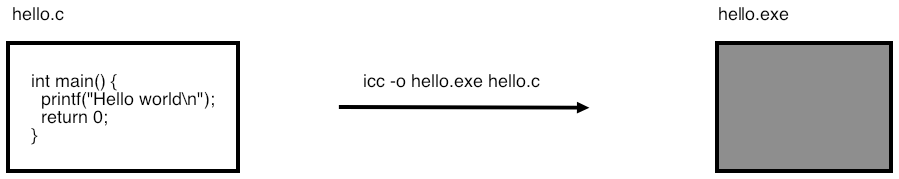
\includegraphics[scale=.5]{compilelink1}
  \caption{Compiling a single source file.}
  \label{fig:compilelink1}
\end{figure}

Let's start with a simple program that has the whole source in one
file.

\srclisting{One file: \n{hello.c}}{compile/c/hello.c}

Compile this program with your favorite compiler; we will use \n{gcc}
in this tutorial, but substitute your own as desired.
\begin{taccnote}
  On TACC clusters, the Intel compiler \n{icc} is preferred.
\end{taccnote}
As a result of
the compilation, a file \indextermtt{a.out} is created, which is the executable.
\begin{verbatim}
%% gcc hello.c
%% ./a.out
hello world
\end{verbatim}
You can get a more sensible program name with the \n{-o} option:
\begin{verbatim}
%% gcc -o helloprog hello.c
%% ./helloprog
hello world
\end{verbatim}
This process is illustrated in figure~\ref{fig:compilelink1}.

\Level 1 {Multiple files: compile and link}

\begin{figure}[ht]
  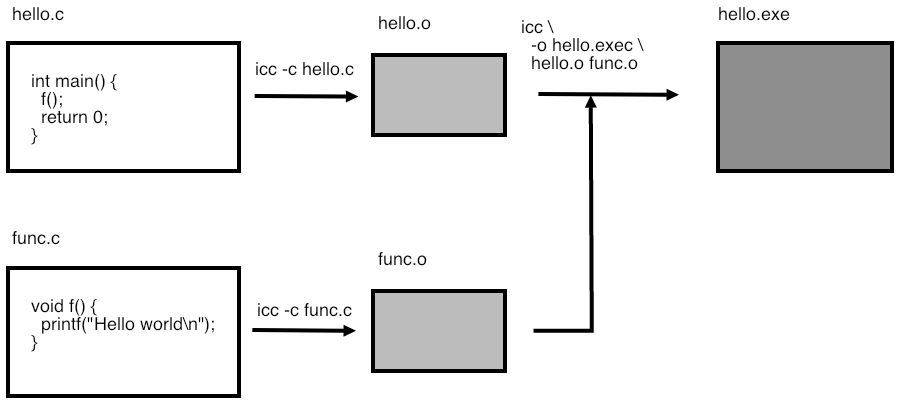
\includegraphics[scale=.5]{compilelink2}
  \caption{Compiling a program from multiple source files.}
  \label{fig:compilelink2}
\end{figure}

Now we move on to a program that is in more than one source file.

\begin{multicols}{2}
  Main program: \n{fooprog.c}
  \cverbatimsnippet{foomain}
  %\lstinputlisting{6compile/fooprog.c}
  \columnbreak
  Subprogram: \n{foosub.c}
  \cverbatimsnippet{foosub}
  %\lstinputlisting{compile/foosub.c}
\end{multicols}

As before, you can make the program with one command.

\snippetmakeoutput{code/compile}{makeoneprogram}

However, you can also do it in steps, compiling each file separately
and then linking them together.
This is illustrated in figure~\ref{fig:compilelink2}.

\snippetmakeoutput{code/compile}{makeseparatecompile}

The \texttt{-c} option tells the compiler to compile the source file,
giving an \indexterm{object file}. The third command then acts as the
\indexterm{linker}, tieing together the object files into an
executable. (With programs that are spread over several files there is
always the danger of editing a subroutine definition and then
forgetting to update all the places it is used. See the `make'
tutorial, section~\ref{tut:gnumake}, for a way of dealing with this.) 

\begin{exercise}
  \label{ex:compile3}

  Exercise for separate compilation. Structure:
\begin{multicols}{2}
  Main program: \n{fooprog.c}
  \strippedinput{code/compile/}{fooprog.c}
  \columnbreak
  Subprogram: \n{foosub.c}
  \strippedinput{code/compile}{foosub.c}
  Add a second subroutine in a second file.
\end{multicols}

  \begin{itemize}
  \item Compile in one:
\begin{verbatim}
icc -o program fooprog.c foosub.c
\end{verbatim}
\item Compile in steps:
\begin{verbatim}
icc -c fooprog.c
icc -c foosub.c
icc -o program fooprog.o foosub.o
\end{verbatim}
What files are being produced each time?
  \end{itemize}
Can you write a shell script to automate this?
\end{exercise}

\Level 1 {Looking into binary files: \texttt{nm}}

Most of a binary file consists of the same instructions that you
coded in C or Fortran, just in machine language, which
is much harder to understand.
Fortunately, you don't need to look at machine language often.
What often interests you about object files is what functions are
defined in it, and what functions are used in it.

For this, we use the \indextermunixdef{nm} command.

Each object file defines some routine names, and uses some others that
are undefined in it, but that will be defined in other object files or
system libraries. Use the \indextermunix{nm} command to display
this:
\begin{verbatim}
[c:264] nm foosub.o
0000000000000000 T _bar
                 U _printf
\end{verbatim}
Lines with \n{T} indicate routines that are defined; lines with \n{U}
indicate routines that are used but not define in this file. In this
case, \n{printf} is a system routine that will be supplied in the
linker stage.

Sometimes you will come across \indextermsub{stripped}{binary} file,
and \indextermunix{nm} will report \n{No symbols}.
In that case \n{nm -D} may help, which displays `dynamic symbols'.

\Level 1 {Compiler options and optimizations}

Above you already saw some \indextermbus{compiler}{options}:
\begin{itemize}
\item Specifying \n{-c} tells the compiler to only compile, and not do
  the linking stage; you would do this in case of separate
  compilation.
\item The option \n{-o} gives you the opportunity to specify the name
  of the output file; without it, the default name of an executable is
  \indextermtt{a.out}.
\end{itemize}

There are many other options, some of them a \emph{de facto} standard,
and others specific to certain compilers.

\Level 2 {Symbol table inclusion}

The \n{-g} option tells the compiler to include the \indexterm{symbol
  table} in the binary.  This allows you to use an interactive
debugger (section~\ref{tut:debug}) since it relates machine
instructions to lines of code, and machine addresses to variable
names.

\Level 2 {Optimization level}

Compilers can apply various levels of
\emph{optimization}\index{compiler!optimization} to your code. The
typical optimization levels are specified as \n{-O0} `minus-oh-zero',
\n{-O1}, \n{-O2}, \n{-O3}. Higher levels will typically give faster
execution, as the compiler does increasingly sophisticated analysis on
your code.

The following is a fairly standard set of options:
\begin{verbatim}
icc -g -O2 -c myfile.c
\end{verbatim}

As an example, let's look at \indexterm{Given's rotations}:
\cverbatimsnippet{givensfun}
Run with optimization level 0,1,2,3 we get:
\begin{verbatim}
Done after 8.649492e-02
Done after 2.650118e-02
Done after 5.869865e-04
Done after 6.787777e-04
\end{verbatim}
\begin{exercise}
  \label{ex:givens-optimize}
  From level zero to one we get (in the above example;
  in general this depends on the compiler) an improvement
  of $2\times$ to $3\times$. Can you find an obvious factor of two?

  Use the optimization report facility of your compiler to see what
  other optimizations are applied. One of them is a good lesson in
  benchmark design!
\end{exercise}

Many compilers can generate a report of what optimizations they perform.

\begin{tabular}{ll}
  compiler&reporting option\\
  clang& \texttt{-Rpass=.*}\\
  gcc&   \texttt{-fopt-info}\\
  intel& \texttt{-qopt-report}\\
\end{tabular}

Generally, optimizations leave the semantics of your code
intact. (Makes kinda sense, not?)  However, at higher levels,
usually level~3, the compiler is
at liberty to make transformations that are not legal
according to the language standard, but that in the majority of cases
will still give the right outcome. For instance, the C~language
specifies that arithmetic operations are evaluated left-to-right.
Rearranging arithmetic expressions is usually safe, but not always.
Be careful when applying higher optimization levels!

\Level 0 {Libraries}
\index{libraries!creating and using|(}

\begin{purpose}
  In this section you will learn about libraries.
\end{purpose}

\begin{figure}[ht]
  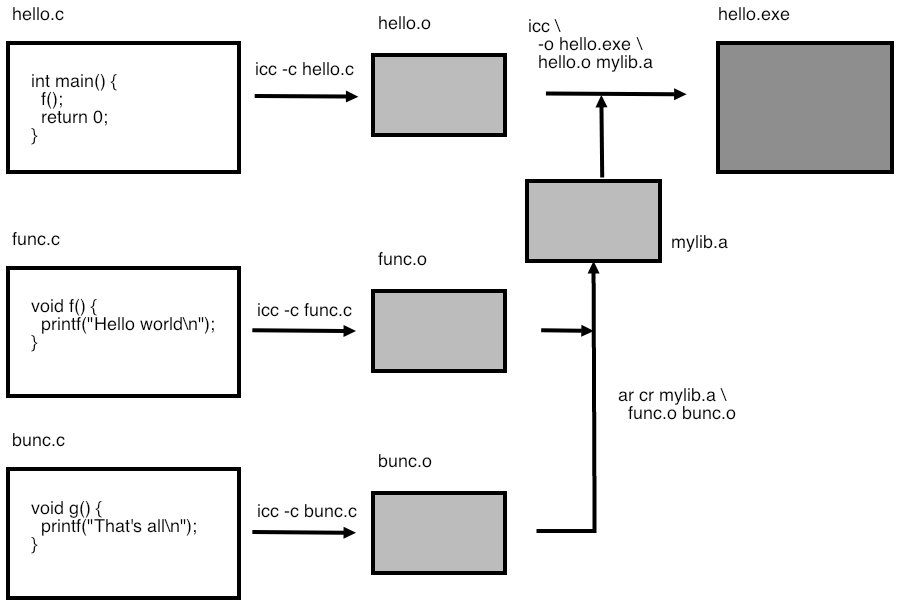
\includegraphics[scale=.5]{compilelink3}
  \caption{Compiling a single source file.}
  \label{fig:compilelink3}
\end{figure}

If you have written some subprograms, and you want to share them with
other people (perhaps by selling them), then handing over individual
object files is inconvenient. Instead, the solution is to combine them
into a library.

\Level 1 {Static libraries}

First we look at
\emph{static libraries}\index{library!static}%
\index{static library|see{library, static}},
for
which the \indexterm{archive utility} \n{ar} is used. A~static library
is linked into your executable, becoming part of it. This may lead to
large executables; you will learn about shared libraries
next, which do not suffer from this problem.

The use of a library to build a program is illustrated
in figure~\ref{fig:compilelink3}.

Create a directory to contain your library (depending on what your
library is for this can be a
system directory such as \n{/usr/bin}), and create the library file
there. 

\snippetmakeoutput{code/compile}{staticprogram}

The \indextermunix{nm} command tells you what's in the library, just
like it did with object files, but now it also tells you what object
files are in the library:
\begin{verbatim}
%% nm ../lib/libfoo.a 

../lib/libfoo.a(foosub.o):
00000000 T _bar
         U _printf
\end{verbatim}

The library can be linked into your executable by explicitly giving
its name, or by specifying a library path:

\snippetmakeoutput{code/compile}{staticprogram}

\Level 1 {Shared libraries}

Although they are somewhat more complicated to use, 
\emph{shared libraries}\index{library!shared}%
\index{shared library|see{library, shared}}
have several advantages. For
instance, since they are not linked into the executable but only
loaded at runtime, they lead to (much) smaller executables. They are
not created with \n{ar}, but through the compiler. For instance:

\snippetmakeoutput{code/compile}{makedynamiclib}

You can again use \indextermunix{nm}:
\begin{verbatim}
%% nm ../lib/libfoo.so 

../lib/libfoo.so(single module):
00000fc4 t __dyld_func_lookup
00000000 t __mh_dylib_header
00000fd2 T _bar
         U _printf
00001000 d dyld__mach_header
00000fb0 t dyld_stub_binding_helper
\end{verbatim}

Shared libraries are not actually linked into the executable;
instead, the executable needs the information where the library
is to be found at execution time. One way to do this is with
\n{LD_LIBRARY_PATH}:
%\indextermunixdefus{LD_LIBRARY_PATH}:

\snippetmakeoutput{code/compile}{dynamicprogram}

Another solution is to have the path be included in the executable:
\begin{verbatim}
%% gcc -o foo fooprog.o -L../lib -Wl,-rpath,`pwd`/../lib -lfoo
%% ./foo
hello world
\end{verbatim}
The link line now contains the library path twice:
\begin{enumerate}
\item once with the \n{-L} directive so that the linker can resolve
  all references, and
\item once with the linker directive \verb+-Wl,-rpath,`pwd`/../lib+ which
  stores the path into the executable so that it can be found at runtime.
\end{enumerate}

Use the command \indextermunixdef{ldd} to get information about what shared libraries
your executable uses. (On Mac OS~X, use \n{otool -L} instead.)


\index{libraries!creating and using|)}


% LocalWords:  Eijkhout unix ascii unicode Matlab hdf hexdump gcc icc
% LocalWords:  cbinwrite cbinwread fbinwrite TACC fooprog foomain de
% LocalWords:  foosub makeoneprogram makeseparatecompile tieing kinda
% LocalWords:  printf Given's givensfun ar staticprogram LD ldd otool
% LocalWords:  makedynamiclib dynamicprogram
